\documentclass{beamer}
\usepackage[utf8]{inputenc}

\usetheme{Madrid}
\usecolortheme{default}
\usepackage{amsmath,amssymb,amsfonts,amsthm}
\usepackage{txfonts}
\usepackage{tkz-euclide}
\usepackage{listings}
\usepackage{adjustbox}
\usepackage{array}
\usepackage{tabularx}
\usepackage{gvv}
\usepackage{lmodern}
\usepackage{circuitikz}
\usepackage{tikz}
\usepackage{graphicx}

\setbeamertemplate{page number in head/foot}[totalframenumber]

\usepackage{tcolorbox}
\tcbuselibrary{minted,breakable,xparse,skins}

\definecolor{bg}{gray}{0.95}
\DeclareTCBListing{mintedbox}{O{}m!O{}}{%
	breakable=true,
	listing engine=minted,
	listing only,
	minted language=#2,
	minted style=default,
	minted options={%
		linenos,
		gobble=0,
		breaklines=true,
		breakafter=,,
		fontsize=\small,
		numbersep=8pt,
		#1},
	boxsep=0pt,
	left skip=0pt,
	right skip=0pt,
	left=25pt,
	right=0pt,
	top=3pt,
	bottom=3pt,
	arc=5pt,
	leftrule=0pt,
	rightrule=0pt,
	bottomrule=2pt,
	toprule=2pt,
	colback=bg,
	colframe=orange!70,
	enhanced,
	overlay={%
		\begin{tcbclipinterior}
			\fill[orange!20!white] (frame.south west) rectangle ([xshift=20pt]frame.north west);
	\end{tcbclipinterior}},
	#3,
}
\lstset{
	language=C,
	basicstyle=\ttfamily\small,
	keywordstyle=\color{blue},
	stringstyle=\color{orange},
	commentstyle=\color{green!60!black},
	numbers=left,
	numberstyle=\tiny\color{gray},
	breaklines=true,
	showstringspaces=false,
}
%------------------------------------------------------------
% Title page info
\title %optional
{4.11.25}
\author % (optional)
{Revanth Siva Kumar.D - EE25BTECH11048}

\begin{document}
	
	\frame{\titlepage}
	
	\begin{frame}{Question}
		Find the distance of the point $\myvec{1,-2,9}$ from the point of intersection of the line
		\[
		\vec{r} = 4\hat{i} + 2\hat{j} + 7\hat{k} + \lambda \myvec{3\hat{i} + 4\hat{j} + 2\hat{k}}
		\]
		and the plane
		\[
		\vec{r}\cdot\myvec{\hat{i} - \hat{j} + \hat{k}} = 10.
		\]
	\end{frame}
	
	
	\begin{frame}{General Formulation}
	The line can be written as
	\begin{align}
	    \vec{r} &= \vec{r}_0 + \lambda \vec{d},
	\end{align}
	where $\vec{r}_0$ is a point on the line, $\vec{d}$ is the direction vector.
	
	The plane equation is
	\begin{align}
	    \vec{n}^T \vec{r} = c,
	\end{align}
	where $\vec{n}$ is the normal vector and $c$ is a constant.
	\end{frame}
	
	
	\begin{frame}{Intersection of Line and Plane}
	Substitute $\vec{r} = \vec{r}_0 + \lambda \vec{d}$ into the plane:
	\begin{align}
	    \vec{n}^T(\vec{r}_0 + \lambda \vec{d}) &= c \\
	    \implies \lambda &= \frac{c - \vec{n}^T \vec{r}_0}{\vec{n}^T \vec{d}}.
	\end{align}
	
	The intersection point is
	\begin{align}
	    \vec{P} = \vec{r}_0 + \frac{c - \vec{n}^T \vec{r}_0}{\vec{n}^T \vec{d}} \vec{d}.
	\end{align}
	\end{frame}
	
	
	\begin{frame}{Distance Formula}
	Let the external point be $\vec{A}$.
	
	Then displacement vector is
	\begin{align}
	    \vec{v} &= \vec{P} - \vec{A}\\
	    \vec{v} &= \vec{r}_0 + \frac{c - \vec{n}^T \vec{r}_0}{\vec{n}^T \vec{d}} \vec{d} -\vec{A}.
	\end{align}
	
	Thus the required distance is
	\begin{align}
	    d &= \|\vec{v}\| = \sqrt{\vec{v}^T \vec{v}}.
	\end{align}
	\end{frame}
	
	
	\begin{frame}{Substitution from Question}
	From the question:
	\begin{align}
	    \vec{r}_0 &= \myvec{4 \\ 2 \\ 7}, &
	    \vec{d} &= \myvec{3 \\ 4 \\ 2}, \\
	    \vec{n} &= \myvec{1 \\ -1 \\ 1}, &
	    c &= 10, \\
	    \vec{A} &= \myvec{1 \\ -2 \\ 9}.
	\end{align}
	\end{frame}
    \begin{frame}{Substitution from Question}
    Compute:
	\begin{align}
	    \vec{n}^T \vec{d} &= \myvec{1 & -1 & 1}\myvec{3 \\ 4 \\ 2} = 1, \\
	    \vec{n}^T \vec{r}_0 &= \myvec{1 & -1 & 1}\myvec{4 \\ 2 \\ 7} = 9, \\
	    \lambda &= \frac{10 - 9}{1} = 1.
	\end{align}
	\end{frame}
	
	
	\begin{frame}{Final Calculation}
	Intersection point:
	\begin{align}
	    \vec{P} &= \myvec{4 \\ 2 \\ 7} + 1\cdot \myvec{3 \\ 4 \\ 2} = \myvec{7 \\ 6 \\ 9}.
	\end{align}
	
	Displacement:
	\begin{align}
	    \vec{v} &= \vec{P} - \vec{A} = \myvec{7 \\ 6 \\ 9} - \myvec{1 \\ -2 \\ 9} = \myvec{6 \\ 8 \\ 0}.
	\end{align}
	
	Distance:
	\begin{align}
	    d &= \sqrt{6^2 + 8^2 + 0^2} = \sqrt{100} = 10.
	\end{align}
	\end{frame}
	
	
	\begin{frame}{Conclusion}
	\textbf{Final Answer: } The required distance is 
	\[
	\boxed{10}
	\]
	\end{frame}
	
	
	\begin{frame}[fragile]{C Code}
	\begin{lstlisting}
#include <stdio.h>
#include <math.h>

// Function to compute distance between A(1,-2,9) and P(7,6,9)
double compute_distance() {
    double A[3] = {1, -2, 9};
    double P[3] = {7, 6, 9};
    double v[3];
    double sum = 0.0;

    for(int i=0; i<3; i++) {
        v[i] = P[i] - A[i];
        sum += v[i]*v[i];
    }

    return sqrt(sum);
}
	\end{lstlisting}
	\end{frame}
	
	
	\begin{frame}[fragile]{Python Code (C Shared Library)}
	\begin{lstlisting}
import ctypes

# Load the shared C library
lib = ctypes.CDLL("./points.so")

# Specify return type
lib.compute_distance.restype = ctypes.c_double

# Call the C function
distance = lib.compute_distance()

print("Distance from (1,-2,9) to intersection point (7,6,9):", distance)
	\end{lstlisting}
	\end{frame}
	
	
	\begin{frame}[fragile]{Python Code (Visualization)}
	\begin{lstlisting}
import numpy as np
import matplotlib.pyplot as plt

# Given point
A = np.array([1, -2, 9])

# Line: r = r0 + lambda*d
r0 = np.array([4, 2, 7])
d = np.array([3, 4, 2])
lambda_vals = np.linspace(-1, 2, 100)
line_points = r0.reshape(3,1) + d.reshape(3,1) * lambda_vals

# Intersection point
P = r0 + d

# Plane: x - y + z = 10
x_plane = np.linspace(-5, 10, 20)
y_plane = np.linspace(-5, 10, 20)
\end{lstlisting}
	\end{frame}
	
	
	\begin{frame}[fragile]{Python code}
    \begin{lstlisting}
        
X, Y = np.meshgrid(x_plane, y_plane)
Z = 10 - X + Y
fig = plt.figure()
ax = fig.add_subplot(111, projection='3d')

# Plot plane
ax.plot_surface(X, Y, Z, alpha=0.3, color='cyan', rstride=1, cstride=1, edgecolor='none')

# Plot line
ax.plot(line_points[0,:], line_points[1,:], line_points[2,:], color='blue', label="Line r=r0+λd")
\end{lstlisting}
	\end{frame}

    \begin{frame}[fragile]{Python code}
    \begin{lstlisting}
# Plot points
ax.scatter(A[0], A[1], A[2], color='red', s=50, label="Point A(1,-2,9)")
ax.scatter(P[0], P[1], P[2], color='green', s=50, label="Intersection P(7,6,9)")

# Dotted line from A to P
ax.plot([A[0], P[0]], [A[1], P[1]], [A[2], P[2]], color='magenta', linestyle='--', label="Distance d")

ax.set_xlabel('X-axis')
ax.set_ylabel('Y-axis')
ax.set_zlabel('Z-axis')
ax.set_title("Distance from Point to Line-Plane Intersection")
ax.legend()
plt.show()
	\end{lstlisting}
	\end{frame}
	
	
	\begin{frame}{Plot}
	    \begin{figure}[H]
	        \centering
	        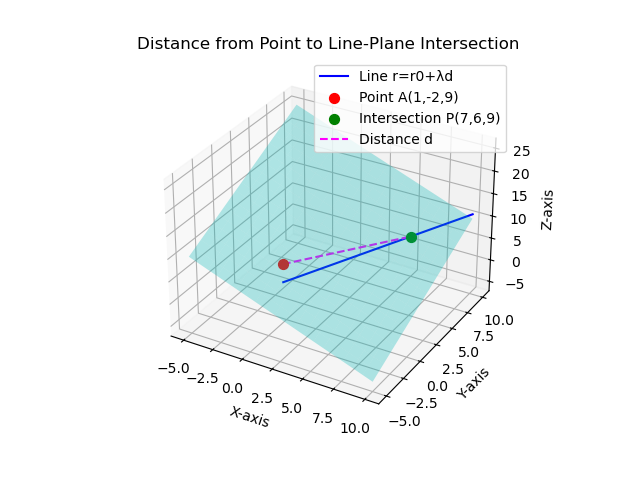
\includegraphics[width=0.7\columnwidth]{figs/Figure_1.png}
	        \caption{3D visualization of point, line, plane, and distance}
	    \end{figure}
	\end{frame}
	
\end{document}
